\documentclass{article}

\usepackage[paper=letterpaper,margin=2.5cm]{geometry} % Set Margins

%% Math and math fonts
\usepackage{amsmath, amsthm, amssymb, amsfonts}
\usepackage{bbm} % for \mathbbm{1}

% date
\usepackage[nodayofweek]{datetime}

% Color
\usepackage{color, xcolor}

% Misc
\usepackage{environ}  % \collect@body in asmmath
\usepackage{graphicx} % \includegraphics options
\usepackage{mdframed} % text boxes
\usepackage{indentfirst} % Indent first paragraph after section header
\usepackage{comment} % Comments
\usepackage{fancyhdr} % Headers and footers

% Tables
\usepackage{array}

% Sub-figures and figure placement
\usepackage{caption}
\usepackage{subcaption}
\usepackage{float} 

% Graphing
\usepackage{pgfplots}
\pgfplotsset{compat=1.17}
\usepackage{tikz}

% Title Placement
\usepackage{titling}
\setlength{\droptitle}{-6em}

%set indent to 
\setlength{\parindent}{0pt}

% Hyper refs
\usepackage{hyperref}
\hypersetup{
    colorlinks=true,
    linkcolor=blue,
    urlcolor  = blue,
    filecolor=magenta,      
    urlcolor=blue,
    citecolor = blue,
    anchorcolor = blue
}

% % Citation management
\usepackage{natbib}
\bibliographystyle{abbrvnat}
\setcitestyle{authordate,open={(},close={)}}

\pagestyle{fancy}

\usepackage[paper=letterpaper,margin=2.5cm]{geometry} % Set Margins

%% Math and math fonts
\usepackage{amsmath, amsthm, amssymb, amsfonts}
\usepackage{bbm} % for \mathbbm{1}

% date
\usepackage[nodayofweek]{datetime}

% Color
\usepackage{color, xcolor}

% Misc
\usepackage{environ}  % \collect@body in asmmath
\usepackage{graphicx} % \includegraphics options
\usepackage{mdframed} % text boxes
\usepackage{indentfirst} % Indent first paragraph after section header
\usepackage{comment} % Comments
\usepackage{fancyhdr} % Headers and footers

% Tables
\usepackage{array}

% Sub-figures and figure placement
\usepackage{caption}
% \usepackage{subcaption}
\usepackage{float} 

% Graphing
\usepackage{pgfplots}
\pgfplotsset{compat=1.17}
\usepackage{tikz}

% Title Placement
\usepackage{titling}
\setlength{\droptitle}{-6em}

%set indent to 
\setlength{\parindent}{0pt}

% Hyper refs
\usepackage{hyperref}
\hypersetup{
    colorlinks=true,
    linkcolor=blue,
    urlcolor  = blue,
    filecolor=magenta,      
    urlcolor=blue,
    citecolor = blue,
    anchorcolor = blue
}

% % Citation management
\usepackage{natbib}
\bibliographystyle{abbrvnat}
\setcitestyle{authordate,open={(},close={)}}

\newcolumntype{M}{>{$}c<{$}} % Define a new column type for math mode


% ----------------------------------------
% TITLE
% ----------------------------------------

\pagestyle{fancy}

\lhead{Creel}
\chead{Section}
\rhead{AMES}

\title{AMES Week 3 Section Notes -- Help for Pset 1}
\author{Andie Creel}

\begin{document}
\maketitle

\section{Example of Solving System of Equations (Q1)}
Consider the system of equations:

\begin{align*}
\text{Equation 1: } & 2x + 3y = 7 \\
\text{Equation 2: } & x - y = 1
\end{align*}

We'll solve this system using the substitution method:

\textbf{Step 1:} Solve Equation 2 for \(x\):
\[x = y + 1\]

\textbf{Step 2:} Substitute the expression from Step 1 into Equation 1:
\[2(y + 1) + 3y = 7\]

\textbf{Step 3:} Solve the resulting equation for \(y\):
\begin{align*}
2y + 2 + 3y &= 7 \\
5y + 2 &= 7 \\
5y &= 5 \\
y &= 1
\end{align*}

\textbf{Step 4:} Substitute the value of \(y\) back into the expression for \(x\) from Step 1:
\[x = y + 1 = 1 + 1 = 2\]

So, the solution to the system of equations is \(x = 2\) and \(y = 1\).\\

\textbf{Things to note for this and Q1 on Pset 1:} Here, the variables are $x,y$ and the parameters are $2,3,7, 1, -1, \text{ and } 1$. On Q1 of the pset, the variables are $N_1, N_2$ and the parameters are $r_1, K_1, r_2, K_2, \alpha, \beta$. The only difference between this example and the pset questions is the difficulty of algebra, and keeping track of all your parameters (easier when your parameters are numbers because they "combine" easily). 

\section{Plotting Exponential Functions (Q2)}

Important to know what the exponential function looks like $f(x) = e^x = exp(x)$ (Figure 1). The exponential function grows SO FAST. \\ $e^3 \approx 20$.\\ $e^5 \approx 150 $.\\ $e^{10} \approx 22K$ \\

\begin{tabular}{c|c}
      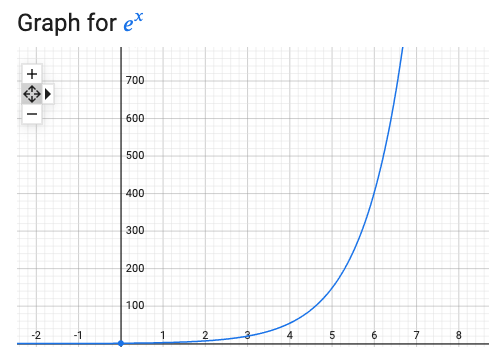
\includegraphics[width=0.45\linewidth]{Screen Shot 2024-09-09 at 4.44.20 PM.png} &  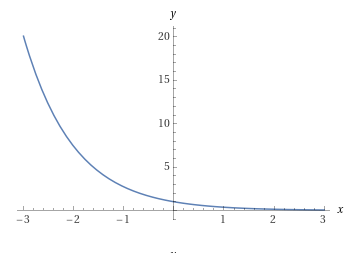
\includegraphics[width=0.45\linewidth]{Screen Shot 2024-09-09 at 5.00.44 PM.png}
\end{tabular}


Now, what if we wanted to plot \[f(x) = e^{-x}?\] Remember that we can rewrite the negative exponent as \[f(x) = \frac{1}{e^x}.\] 
So, $1/e^x$ is going to approach $1/\infty$ really fast because $e^x$ approaches $\infty$ really fast. \textit{What's $1/\infty$?}\\

On Q2, need to think about how your Y-intercept won't be 1 because of the $A$ in the equation, and how the limit won't be 0 because of the $A$ as well. 

\section{Plotting Second Order Functions (Q2)}
Plot $G(x) = ax - x^2 +b$. 

\begin{enumerate}
    \item First, need to know that $-x^2$ is an upside down parabola.
    \item The $b$ is going to shift it up. The $ax$ is going to shift it to the right (assuming $a$ is positive). 
    \item Find the y intercept  
    \item What does $x$ need to equal for $G(x) = b$? One value is the intercept, but there is a second value for $x$ because of the parabola shape. Set $ax-x^2=0$ because the is similar to how we got the y-intercept earlier? 
\end{enumerate}

\section{Cobb-Douglas level sets (Q5)}


Consider the function 
\begin{align*}
    F(x_1, x_2) = x_1^{1/2} x_2^{1/2}
\end{align*}
$F(x_1, x_2)$ maps from $R^2$ to $R^1$, 
\begin{align*}
    R^2 \to R^1.
\end{align*}

To visualize $F(x_1, x_2)$ we need to do it in $R^3$ (3-D) because we need a dimension for both inputs and the output.\\

To visualize a $n$ dimensional function you need a $n+1$ dimensions because you need an additional dimension for the output.

\begin{figure}[htp]
    \centering
        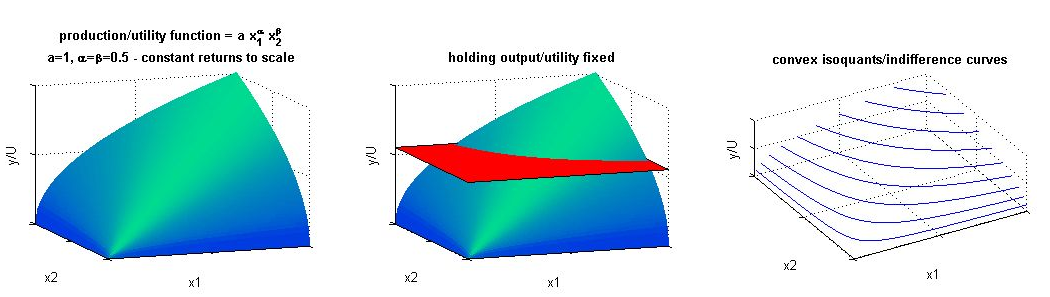
\includegraphics[width=1\textwidth]{Screen Shot 2023-09-18 at 2.03.06 PM.png}
    % \caption{convex and concave }
    % \label{fig:sample}
\end{figure}

Source: \url{https://www2.hawaii.edu/~fuleky/anatomy/anatomy.html}\\



If a function is in $R^2$ (\textit{i.e.} it takes two inputs) then you must evaluate if  the function is convex or concave in $R^3$. That will determine if the function is convex or concave. But then if you graph you function in $R^2$ space (meaning you're not using an additional dimension for the output) the function may look convex or concave in the lower dimension. Despite how it looks in the lower dimension, you must determine if it's quasi-convex or quasi-concave from the higher dimension.  \\

If the function is convex in $R^3$ (\textit{e.g.} it looks like a bowl), when you graph it in $R^2$ it's quasi-convex. If the function is concave in $R^3$ (\textit{e.g.,} it looks like a hat), when graphed in $R^2$ it's quasi-concave. \\

\textit{Verbally explain what would happen if you set $ F(x_1, x_2)$ to a constant $C$ and solve for $ x_1 = g(x_2, C)$. Is $g(\cdot)$ convex or concave?}



Let utility be $ U(x,y) = x^\beta y^{1-\beta}$

\begin{enumerate}
    \item What do the level sets look like in the $\mathbf{R}^{++}$ (aka 2D space)?
    \item Quasi concave or quasi convex? 
    \item Where is utility better off? 
\end{enumerate}


\section{Log Rules (Q6)}
Consider the equation 
\begin{align*}
    y = \alpha x e^{\beta x}\nu
\end{align*}

where $y$ is an endogenous-variable (determined by the system \textit{aka} dependent variable), $x$ is a variable (aka independent variable), $\alpha$ is an exogenous parameter, $\beta$ is an exogenous parameter, and $\nu$ is measurement error.\\

You want to use log rules so that you can get this to look like an equation where you could use linear regression to estimate $\alpha$ and $\beta$. That mean we want an endogenous variable that's a function of a constant, a linear term with the dependent variable, and an error term.

\begin{align*}
    \log(y) &= \log(\alpha x e^{\beta x}\nu) \\
    \log(y) &= \log(\alpha) + \log(x) + \log(e^{\beta x}) +\log(\nu)\\
    \log(y) &= \log(\alpha) + \log(x) + \beta x \log(e) + \log(\nu)\\
    \log(y) &= \log(\alpha) + \log(x) + \beta x + \log(\nu)\\
    \log(y) - \log(x) &= \log(\alpha) + \beta x + \log(\nu) \\
    \log(y/x) &= \log(\alpha) + \beta x + \log(\nu)
\end{align*}


\end{document}